%!TEX root = ../dissertation.tex

\chapter{Implementation}
\label{chapter:implementation}
To demonstrate the feasibility and validity of the proposed architecture, a proof-of-concept implementation has been developed by means of extending an existing \gls{SDN} controller and integrating a Linux kernel module for clustering.\\
%
The requirements set for the controller selection were controller completeness, popularity and availability of source code, which lead to a final decision between OpenDaylight \cite{OpenDaylight} and Floodlight \cite{Floodlight}\cite{Kreutz2014}\cite{ControllerComparison}.
%Justify choice of Floodlight
While both OpenDaylight and Floodlight are modular open-source \gls{SDN} controllers implemented in Java, highly popular and supported by major players in the networking industry \cite{OpenDaylight}\cite{Floodlight}, at the time of the decision, Floodlight, which was at version 1.1, had a more stable implementation when compared with the OpenDaylight, which was at release Helium.
OpenDaylight also offers support for multiple Southbound Interface protocols which, while falling outside the scope of this work, would render the architecture of the platform more complex than that of Floodlight, and would therefore add more complexity to the implementation.
For these reasons, Floodlight was chosen as a basis for the implementation of the proof-of-concept for the proposed architecture.\\
%
\section{Elastic SDN controller cluster}
\label{section:SDN-controller-cluster-implementation}
% Floodlight
Floodlight is a modular implementation of an \gls{SDN} controller developed by Big Switch Networks using the Java language, and is currently in version 1.1.
Floodlight shares its core implementation with Big Switch Networks's own Big Network Controller \cite{Floodlight}.
It offers stable support for OpenFlow versions 1.0 and 1.3 and experimental support for versions 1.1, 1.2 and 1.4 through OpenFlowJ Loxi, a library that encapsulates the OpenFlow protocol and exposes functionality through a protocol version agnostic \gls{API} \cite{LoxiGen}.\\
Floodlight's architecture is highly modular, composed by a base \emph{Module Loading System} that loads a set of registered modules, allowing for the establishment of inter-module dependencies as well as service exposure and consumption by registered modules \cite{FLArch}.
There are a set of \emph{Controller Modules} which implement core \gls{SDN} controller functionality which is then either exposed by service \glspl{API} or by propagating as events to registered listener modules, thus enabling an event-driven programming model.
These modules implement features such as OpenFlow switch management connection handling (FloodlightProvider and OFSwitchManager modules), inter-switch link discovery through \gls{LLDP} and \gls{BDDP} (LinkDiscoveryManager module), network host discovery and tracking through packet-in inspection (DeviceManagerImpl module) and network topology and routing service (TopologyService module).\\
Floodlight defines a unique device as a \gls{VLAN}/\gls{MACAddress} pair and considers that there may be at most one attachment point per network domain \cite{FLArch}.
In order to maintain compatibility the same principles were taken into consideration for the implementation of the proof-of-concept.\\
%NOTE: DeviceManagerImpl "By default the entity classifier uses MAC address and VLAN to identify a device. These two properties will define what is unique as a device. (...) A device can have as many as one attachment point per OpenFlow island, where an island is defined as a strongly connected set of OpenFlow switches talking to the same Floodlight controller."
%
\subsection{Proof of concept implementation}
\label{subsection:poc-module}
%
% Highlevel description
The proof-of-concept implementation followed Floodlight's architectural design.
A floodlight module was therefore implemented, encapsulating the clustering mechanisms detailed in Chapter \ref*{chapter:architecture} Section \ref{section:SDN-controller-cluster} and providing both \glspl{API} and triggering events to registered listeners.
The main building blocks composing the developed module, depicted in Figure \ref{fig:amorphous_block_diagram}, are as follows:
%
\begin{figure}
	\centering
	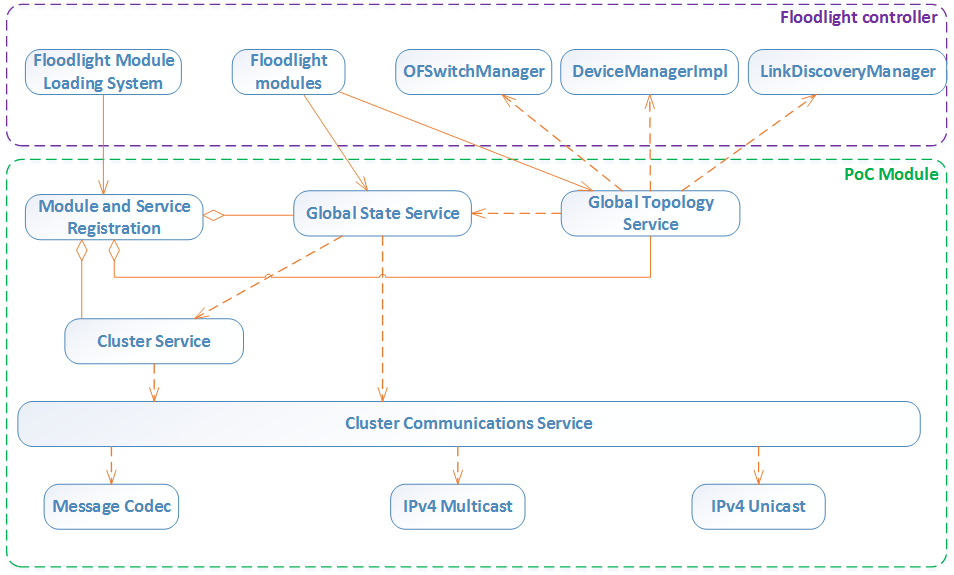
\includegraphics[scale=0.65]{amorphous_block_diagram}
	\caption{Proof of concept implementation high level block diagram}
	\label{fig:amorphous_block_diagram}
\end{figure}
%
\begin{itemize}
	\item \textbf{Module and Service registration:} Handles all the tasks necessary to integrate with the Floodlight controller, including component initialization, declaring dependencies and exposing the services provided by both Global State Service and Global Topology Service by implementing the IFloodlightModule interface, which is then used by the Floodlight Module Loading System to register and execute the module.
	%
	\item \textbf{Global State Service:} Handles the global state of the \gls{MIB} and exposes an \gls{API} to provide message exchange between Floodlight modules executed in different instances of the cluster, therefore allowing for the extension and enhancement of the distributed environment properties to module specific implementations. The message exchange \gls{API} provided is based on the concept of named message queues, in which a module registers in a queue and is allowed to send messages to, and listen for, incoming messages on the queue. This module depends on the Cluster Communications Service to exchange messages with peer controller instances and on the Cluster Service in order to determine the address of the destination peer and whether or not a peer is a member of the cluster.
	%
	\item \textbf{Global Topology Service:} Locally, it provides the same services as the TopologyService module by exposing an \gls{API} to be consumed by other Floodlight modules and triggering events upon topology changes, using however the Global State Service's \gls{MIB} instead of the local \gls{MIB}. It also listens for local topology changes, such as new OpenFlow switch connections, new inter-switch links and hosts, updating its \gls{MIB} and propagating the changes to peer instances accordingly. This block registers to a special queue in Global State Service reserved for the exchange of the messages specified in Table \ref{table:cluster-message-spec} under the scope of \gls{MIB} update. All messages queued for sending through the exposed \gls{API} are sent encapsulated (and de-encapsulated when received before being registered to the corresponding queue) within a special purpose container message that holds properties such as the queue identifier.
	%
	\item \textbf{Cluster Service:} This block is responsible for all the clustering logic such as that of the registration of peer cluster instances (including the registration of the local instance with existing ones) described in Chapter \ref*{chapter:architecture} Section \ref{section:SDN-controller-cluster} and the exchanging and processing of all the messages stated in Table \ref{table:cluster-message-spec} under the scope of cluster membership. Messages are sent and received using the \gls{API} provided by the Cluster Communications Service.
	%
	\item \textbf{Cluster Communications Service:} Encapsulates all of the network communication details, providing a unified \gls{API} to both Cluster Service and Global State Service, thus enabling them to send and receive messages to and from peer controller instances. The messages are encoded/decoded to a suiting transmission format by the Message Codec block, and then sent and received by the network access specific implementations. The network access is done using \gls{IPv4} since it is the most widespread network protocol. The network access specific implementations are contained in the IPv4 Multicast and IPv4 Unicast blocks, allowing for the easy replacement of the network protocol used simply by implementing new blocks that expose the same \gls{API}.
	%
	\item \textbf{Message Codec:} Encodes and decodes messages to a suitable format to be sent through the network, which is essentially an array of bytes. In this implementation, the method chosen to encode/decode is the serialization of Java objects, however, any other method can be implemented such as \gls{JSON} or otherwise a special purpose Application Layer\footnote{Considering the \gls{OSI} model} protocol in order to make messages compatible with any \gls{SDN} controller implementation, regardless of the programming language it was developed in.
	%
	\item \textbf{IPv4 Multicast:} All of the \gls{IPv4} multicast implementation is contained within this block. The multicast group used for this implementation is 224.0.1.20, which is a special group address reserved for private experiments \cite{ReservedMulticastGroups} within the multicast addresses block for portocol traffic that is allowed to be forwarded through the internet \cite{rfc5771}.
	%
	\item \textbf{IPv4 Unicast:} This block implements all of the \gls{IPv4} unicast using only \gls{TCP} as it provides guaranteed delivery independently of message size.
\end{itemize}
%
%TODO: Lamport clocks to guarantee causal consistency and avoid loss of information during the sync process (message buffer)
%
% Optimizations
The group communication paradigm specified in Chapter \ref*{chapter:architecture} Section \ref{section:SDN-controller-cluster} is implemented using the \gls{IPv4} multicast mechanism provided by the IPv4 Multicast block, which presented an additional challenge as \gls{IPv4} multicast does not provide a connection oriented communication, therefore requiring for manual fragmentation, ordering and reassembly of messages with size greater than the \gls{MTU}.
In order to overcome this limitation, without going into complex message delivery implementations and while still keeping the desired properties of group communication, a workaround was implemented in the Cluster Communications Service block in which if the size of a message targeting all cluster members is large enough not to fit into a single packet (in which case the IPv4 Multicast block will raise an exception), instead of using the multicast mechanism, unicast \gls{TCP} sessions are established to all registered clustered members, conveying the message through these sessions.
All of the messages specified in Table \ref{table:cluster-message-spec}, within the scope of cluster membership and targeted at the whole cluster, are guaranteed to fit in a message which size is lesser than the \gls{MTU} and are therefore not affected by this workaround, thus keeping the group communication properties required for cluster formation and maintenance intact.\\
In order to reduce the amount of data transmitted and at the same time provide a fail recovery mechanism, the Join cluster and Instance health messages defined in Table \ref{table:cluster-message-spec} were merged into the a single message (Join cluster), having each instance the responsibility of differentiating the message purpose according to whether the instance sending the message was already registered (in which case a timestamp indicating the last time the instance reported activity is updated) or not (in which case the registration process is executed).\\
%
In order for inter-switch links connecting OpenFlow switches controller by different instances to be properly detected and registered into the global topology, the LinkDiscoveryManager module had be modified in such a way that the incoming \gls{LLDP} packets sent by other controller instances are processed according to the topology made available by the Global topology Service instead.
This represents the only change required to the Floodlight core modules in order for the proof-of-concept implementation to work.
%
\subsection{Distributed network policy module}
\label{subsection:poc-application}
%
Floodlight comes bundled with a set of network applications that provide network policy functionality out of the box.
One of the bundled applications is the Forwarding module, which implements a forwarding policy that permits all flows to go through the network (also known as permit from any to any), installing the necessary flow entries in a reactive fashion \cite{FLFwd}.\\
The nature of this module makes it a perfect test subject for the proposed architecture, however, in order to better demonstrate the full potential of the proposed architecture this module was extended to take advantage of the inter-instance communication mechanism provided by the Global State Service so that the forwarding policy is only computed on the \gls{SDN} controller instance managing the OpenFlow switch to which the device that initiates the flow is connected to. Controller instances managing other OpenFlow switches in the path that the flow takes to traverse the network are simply instructed which flow entries to add to which switches instead of having to compute the policy by themselves.
This approach increases scalability as the computational cost of determining the actions to be performed for any given flow is only inflicted in one controller instance, leaving other controller instances free to compute the flows being admitted into the network through OpenFlow switches that they control directly.\\
This extended version of the Forwarding module, registers to a queue named after itself using the Global State Service \gls{API} which will be used to exchange messages to coordinate policy programming actions throughout the network.
Upon receiving a Packet-In for a packet that hit the table miss flow, it invokes the \gls{API} of the Global Topology Service in order to determine if the destination device is already known in the topology (at global scope) and if so which is the shortest path between the source and destination devices.
Should the destination device be unknown to the topology, the packet is flooded to all ports of the corresponding broadcast domain in the local OpenFlow switch and the process terminates.
If however the destination is known in the global topology, it takes the path computed by the Global Topology Service and in turn computes the flow entry to be programmed in each OpenFlow switch pertaining to path and sends out Flow Programming Request messages to the controller instances managing the involved OpenFlow switches that are not locally managed.
Flow Programming Requests are then processed by the receiving instances which notify the instance that sent it with a Flow Programming Confirmation message upon completion.
The instance that computed the policy is only allowed to program the flow entry in the OpenFlow switch that triggered the Packet-In, after receiving Flow Programming Confirmation messages from all remote instances involved, thus making sure that there will be no other Packet-In triggered in the path.
%
\section{Request Router}
\label{section:request-router-implementation}
The request router component was implemented by integrating Linux virtual machines running Linux kernel 3.16 compiled with the \gls{IPVS} module, with the Elastic \gls{SDN} controller cluster.
The \gls{IPVS} module, pertaining to the \gls{LVS} Project, provides an efficient kernel-mode \gls{OSI} layer 4 switching facility, suited to load balance client connections between several clustered servers \cite{LVS}.
The implementation of the \gls{anycast} communication paradigm assumes that the management network infrastructure, to which the management interfaces of OpenFlow switches and \gls{SDN} controller instances are connected to, supports the \gls{BGP} routing protocol and is able to establish \gls{BGP} peering with the request router instances.
The configuration of the management network infrastructure is not within the scope of this work.
%

\subsection{Linux Virtual Server (LVS)}
\label{subsection:LVS-implementation}
%TODO: Linux LVS
The \gls{LVS} project, in particular the \gls{IPVS} module, provides an out of the box load balancing facility for client-server applications connecting through the network and using the \gls{IPv4} stack.
This module, implemented as a kernel module, introduces minimal overhead in the client-server communication and can be deployed as a cluster, in which mode forwarding states will be synchronized between cluster members, thus allowing for the required infrastructure resiliency seeing that a request router instance failure will not impact normal operation as its peer instance is able to take over the forwarding function seamlessly \cite{IPVSSync}.\\
%
%TODO: IPVS modes http://www.linuxvirtualserver.org/how.html : Because of DST -> VS/DR
The load balancing is performed at the Transport Layer of the \gls{OSI} model, supporting both \gls{UDP} and \gls{TCP} protocols.
IPVS receives the connection data from the client for a configured service cluster and forwards it to the one of the servers available for that cluster in one of three possible ways \cite{IPVSHow}:
\begin{itemize}
	\item In \textbf{\gls{NAT} mode}, \gls{IPVS} terminates the client connection and initiates a new connection with the service cluster instance determined by the load balance algorithm, forwarding all the packets received from the client to the server, masquerading however the source \gls{IPAddress}, effectively forcing data communications to go through the load balancer in both ways. While this mode offers the advantage of allowing the service cluster servers to be located anywhere on the network and requiring no configuration on the clients nor the servers, it has limited scaling capabilities as \gls{NAT} itself is limited when it comes to scaling
	%
	\item In \textbf{IP Tunneling mode}, \gls{IPVS} does not terminate the client-server communication and instead encapsulates the data being received from the client inside an IP-IP packet and forwards it to the service cluster instance determined by the load balance algorithm. This mode also offers the advantage of allowing the service cluster servers to be located anywhere on the network, requiring however that the servers support the IP-IP tunneling (which introduces minimal overhead) and the configuration of loopback interfaces with the service cluster \gls{IPAddress} in all of the service cluster servers and disallow \gls{ARP} on that loopback. It is however much more scalable than \gls{NAT} mode, since this mode does not perform \gls{NAT} nor does it process packets coming from the server to the client.
	%
	\item In \textbf{Direct Routing mode}, \gls{IPVS} behaves essentially in the same way as in the IP Tunneling mode, however, instead of performing encapsulation, the load balancer is required to be on the same \gls{OSI} layer 2 as the service cluster servers, forwarding the packets received by the client directly to the service cluster instance determined by the load balance algorithm. While this mode offers the same advantages as the IP Tunneling mode and without the IP Tunneling drawback, the requirement of being in the same \gls{OSI} layer 2 as the service cluster server represents a limitation in terms of solution design.
	%
\end{itemize}	
%
Both IP Tunneling and Direct Routing modes met the requirements set for the request router component.
Although for the purpose of this implementation Direct Routing has been chosen due to constraints with the deployment target, IP Tunneling mode should be used instead as it does not limit the deployment topology and IP-IP tunneling is natively supported in modern Linux kernels, requiring only that management network routers have the \gls{RPF} feature disabled.
It is worth to note however that the forwarding mode is determined by server and not by service cluster, which means that it is possible to use more than one of these modes simultaneously for different servers in the same service cluster.\\
%
IPVS also offers a number of load balancing algorithms that can be used to determine to which service cluster instance the client connection should be forwarded to:
%
\begin{itemize}
	\item The \textbf{Round Robin} algorithm iterates through the configured servers, equally distributing client connections to each server.
	%
	\item The \textbf{Weighted Round Robin} algorithm allows the definition of weights per server, which are then taken into account when assigning client connections, such that servers with higher weight are assigned more connections.
	%
	\item The \textbf{Least-Connections} algorithm assigns new client connections to the server with least active connections.
	%
	\item The \textbf{Weighted Least-Connections} algorithm is the default algorithm and like the Weighted Round Robin it allows for the definition of weights per server. It then assigns new client connections to the server with the lowest Connections to Weight ratio.
	%
	\item The \textbf{Locality-Based Least-Connections} algorithm assigns incoming connections to the same server if it is not overloaded or unavailable, in which case it assigns the connection to another server with fewer connections.
	%
	\item The \textbf{Locality-Based Least-Connection with Replication} algorithm defines a server set that can serve the client's request and forwards the packets to the server in that set with least active connections. If all servers in the set are overloaded, a new server belonging to the service cluster is added to the set of servers that can serve the client and the packets are forwarded to that server.
	%
	\item The \textbf{Destination Hashing} algorithm consistently assigns server by looking up a hash table using the service cluster \gls{IPAddress} as key.
	%
	\item The \textbf{Source Hashing} algorithm consistently assigns server by looking up a hash table using the client's \gls{IPAddress} as key.
	%
	\item The \textbf{Shortest Expected Delay} algorithm assigns client connections to the server that is expected to have the shortest delay, which is estimated by $\frac{(C + 1)}{U}$ where $\mathit{C}$ is the number of connections for the server and $\mathit{U}$ the Weight assigned to the server.
	%
	\item The \textbf{Never Queue} algorithm assigns client connections to one of the idling servers. Should there be no idling server the Shortest Expected Delay is used to assign a server.
	%
\end{itemize}
%
The optimal algorithm, according to the requirements set for the request router, would be the Source Hashing since it guarantees a deterministic load balancing decision.
However, for the purposes of testing this implementation using a network emulator, the Least Connections algorithm was instead chosen since the Source Hashing algorithm would always assign the same server because the source \gls{IPAddress} would always be the same for all OpenFlow switches (that of the emulator).
%
\subsection{Elastic Cluster Integration}
\label{subsection:elastic-cluster-integration-implementation}
The request router must integrate with the \gls{SDN} controller elastic cluster in order to determine the set of active controller instances to which it can forward OpenFlow switch connections.
To do that, a new component was developed, much like the developed Floodlight module, joining also the same multicast group in order to receive Join messages through which it infers the active set of controller instances.
Because the message encondig/decoding is performed using Java's object serialization, this components implementation necessarily had to be made using the Java language as well.
The building blocks of the component are depicted in Figure \ref{fig:rr_block_diagram} and are as follows:
%
\begin{figure}
	\centering
	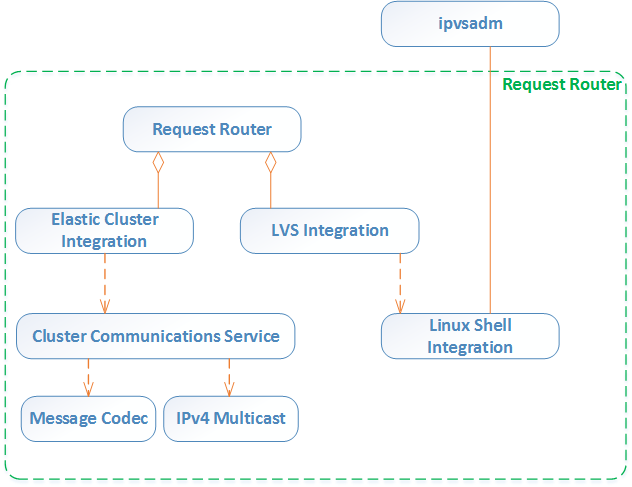
\includegraphics[scale=0.65]{rr_block_diagram}
	\caption{Request Router integration component high level block diagram}
	\label{fig:rr_block_diagram}
\end{figure}
%
\begin{itemize}
	\item \textbf{Request Router:} This block implements all of the load balance logic, handling events generated by the Elastic Cluster Integration and triggering the necessary configuration changes to \gls{IPVS} through the LVS Integration block.
	%
	\item \textbf{LVS Integration:} This block handles the necessary parsing and command issuing with the ipvsadm tool in order to ensure the correct configuration of \gls{IPVS}. 
	%
	\item \textbf{Linux Shell Integration:} An abstraction layer to allow for the execution of Linux shell commands.
	%
	\item \textbf{Elastic Cluster Integration:} This block encapsulates the same cluster membership logic present in the Cluster Service block of the Floodlight elastic clustering module, and is intended to detect cluster member changes and trigger adequate events to the Request Router block.
	%
	\item \textbf{Cluster Communications Service:} Implements essentially the same logic for listening to cluster messages as its homologous block in the Floodlight elastic clustering module.
	%
	\item \textbf{Message Codec:} Implements exactly the same logic as its homologous block in the Floodlight elastic clustering module.
	%
	\item \textbf{IPv4 Multicast:} Implements exactly the same logic as its homologous block in the Floodlight elastic clustering module.
	%
\end{itemize}
%
The component interfaces with the \gls{IPVS} module through ipvsadm, a command line tool design to control \gls{IPVS}, enabling the creation of service clusters and the addition and removal of servers from service clusters.
To do so, the developed component launches new processes for each execution of the ipvsadm tool necessary and parses its output in order to extract status information and command execution success.
%
\subsection{Anycast routing}
\label{subsection:anycast-implementation}
%TODO: Anycast mechanism: BGP ECMP (Quagga) + Loopback on Controllers + disable RPF on core routers
The request router anycast communication paradigm is implemented by adding a third component to the solution, the Quagga Routing Suite.
The Quagga Routing Suite is a routing software suite that implements several routing protocols such as \gls{RIP}, \gls{OSPF}, \gls{IS-IS} and \gls{BGP} as well as the \gls{MPLS} Label Distribution Protocol and \gls{BFD}.\\
%
The anycast communication paradigm is achieved by having the request router instances establish a \gls{BGP} session with the closest management network router and announcing the cluster \gls{IPAddress} to which OpenFlow switches will establish management connections to.
In practice, this means that each router in the management network will have routes to the cluster \gls{IPAddress} that have the next-hop defined as whichever request router instance is closer to them, and as expected different routers in different network regions will have different next-hop defined for that route.
The \gls{ECMP} feature of \gls{BGP} is also used to guarantee that load balancing is also achieved between request router instances, as it allows management network routers to hold multiple active routes for the same destination through different next-hops, thus providing the mechanism to load balance between multiple request router instances provided that they are at the same routing distance.\\
%
To improve the robustness of the solution and minimize convergence time in case of a request router instance failure, \gls{BFD} is also used.
\gls{BFD} is a Hello protocol intended to provide fast failure detection of a network path between two systems regardless of which component might have failed \cite{rfc5880}.
When \gls{BFD} is combined with \gls{BGP} the time it takes to expire a route for a next-hop that is no longer available is reduced from minutes to microseconds \cite{rfc5880}\cite{rfc4271}.
